\documentclass[11pt]{beamer}
%\usetheme{Warsaw}
\usetheme{Antibes}
\usepackage{fancybox}
\usepackage{beamerthemesplit}
\usepackage{graphicx}
\usepackage{xcolor}
\usepackage{url}
\usepackage{ulem} % Needed to produce double underlining using \uuline.
\setbeamertemplate{footline}[page number]{}
\setbeamertemplate{navigation symbols}{}
%\setbeamertemplate{footline}[text line]{}

\definecolor{olive}{rgb}{0.3, 0.4, .1}
\definecolor{fore}{RGB}{249,242,215}
\definecolor{back}{RGB}{51,51,51}
\definecolor{title}{RGB}{255,0,90}
\definecolor{dgreen}{rgb}{0.,0.6,0.}
\definecolor{gold}{rgb}{1.,0.84,0.}
\definecolor{JungleGreen}{cmyk}{0.99,0,0.52,0}
\definecolor{BlueGreen}{cmyk}{0.85,0,0.33,0}
\definecolor{RawSienna}{cmyk}{0,0.72,1,0.45}
\definecolor{Magenta}{cmyk}{0,1,0,0}


\title{{Synchronous Dynamical Systems on}\\ \smallskip
       {Directed Acyclic Graphs (DAGs):} \\ \smallskip  
       {Complexity and Algorithms}
}

\date{}

%%%%%%%%%%%%%%%%%%%%%%%%%%%%%%%%%%%%%%%%
%%%
%%% Symbols needed for dynamical system definitions.
%%%
\newcommand{\cals}{\mbox{$\mathcal{S}$}}
\newcommand{\calc}{\mbox{$\mathcal{C}$}}
\newcommand{\calcp}{\mbox{$\mathcal{C'}$}}

%% \newcommand{\QED}{\hfill\mbox{\hfill\rule{2mm}{2mm}}}
\newcommand{\bbb}{\mbox{$\mathbb{B}$}}
\newcommand{\cala}{\mbox{$\mathcal{A}$}}
\newcommand{\calcdp}{\mbox{$\mathcal{C}^{''}$}}
\newcommand{\calco}{\mbox{$\mathcal{C}_1$}}
\newcommand{\calct}{\mbox{$\mathcal{C}_2$}}
\newcommand{\calcv}{\mbox{$\mathcal{C}_v$}}
\newcommand{\calf}{\mbox{$\mathcal{F}$}}
\newcommand{\calp}{\mbox{$\mathcal{P}$}}
\newcommand{\calso}{\mbox{$\mathcal{S}_1$}}

\newcommand{\tupv}{\mbox{$t_{\mathrm{up}}(v)$}}
\newcommand{\tdownv}{\mbox{$t_{\mathrm{down}}(v)$}}

\newcommand{\pre}{\textsc{Pre}}
\newcommand{\npre}{\textsc{\#Pre}}

\newcommand{\fpe}{\textsc{Fpe}}
\newcommand{\nfpe}{\textsc{\#Fpe}}

\newcommand{\majd}{\mbox{$\lceil (d+1)/2 \rceil$}}

\newcommand{\cpsp}{\mbox{\textbf{PSPACE}}}
\newcommand{\ccnp}{\mbox{\textbf{Co-NP}}}


%%%
%%% End of symbols needed for dynamical system definitions.
%%%
%%%%%%%%%%%%%%%%%%%%%%%%%%%%%%%%%%%%%%%%


\begin{document}

%% \newcommand{\rgreen}[1]{{\color{green!80}#1}}

\frame[squeeze,containsverbatim]{
%\titlepage
\vspace*{-0.25in}
\begin{center}
\textcolor{blue}{\large{\textbf{Synchronous Dynamical Systems 
                 on Directed}}} \\ \smallskip
\textcolor{blue}{\large{\textbf{Acyclic Graphs (DAGs): Complexity and Algorithms}}}
\end{center}

\begin{center}
\textbf{Daniel J. Rosenkrantz$^{1,2}$~~~ Madhav V. Marathe$^{1,3}$}\\ \smallskip
\textcolor{dgreen}{\textbf{S. S. Ravi}}$^{1,2}$~~~ 
\textbf{Richard E. Stearns$^{1,2}$} \\ \smallskip
\end{center}

%\smallskip

\footnotesize{
\textcolor{blue}{
%$^1$Network System Science and Advanced Computing (NSSAC) Division,
$^1$Bioinformatics Institute and Initiative,
University of Virginia,\newline
Charlottesville, VA} %%\smallskip
}

\medskip

\footnotesize{
\textcolor{blue}{
$^2$Department of Computer Science,
University Albany -- State University of New York,
Albany, NY}  %%\smallskip
}

\medskip

\footnotesize{
\textcolor{blue}{
$^3$Department of Computer Science,
University of Virginia, Charlottesville, VA} %%\smallskip
}

\medskip%%\bigskip

\noindent
\footnotesize{
\textcolor{magenta}{\textbf{Email:}}~
    {\texttt{drosenkrantz@gmail.com, marathe@virginia.edu}},\\
   \hspace*{0.5in}{\texttt{ssravi0@gmail.com,  thestearns2@gmail.com}}
}

\bigskip

\noindent
\footnotesize{
\textbf{Acknowledgment:}~ This work was partially supported by NSF Grants
IIS-1633028 (BIG DATA),
CMMI-1745207 (EAGER),
OAC-1916805 (CINES),
CCF-1918656 (Expeditions) and
IIS-1908530.
}

} %%End of title page.


\frame[containsverbatim]{
\frametitle{Talk Outline}

\begin{enumerate}
\item Basics of Discrete Dynamical Systems on DAGs \medskip

\item Previous Work \medskip

\item Problems Considered \medskip

\item Our Main Contributions\medskip

%\item Summary and Future Work \medskip
\item Future Work \medskip

\end{enumerate}
}
%%%%%%%%%%%%%%%%%%%%%%%%%%%%%%%%%%%%%%%%%%%%

\frame[squeeze,containsverbatim]{
\frametitle{Discrete Dynamical Systems on DAGs: Basics}

A \textbf{Discrete Dynamical System on a DAG} ~\cals{} consists of\\
\smallskip
\begin{itemize}
\item An underlying DAG $G(V,E)$.  \medskip

\item \textbf{Nodes:}~ Agents in the system. \medskip

\item \textbf{Edges:}~ Permissible local interactions.  \medskip

\item State values for nodes from a finite domain \bbb{}  \\
      (e.g., \textcolor{dgreen}{\textbf{\bbb{} = \{0,~1\}}}). \medskip

\item A \textbf{local transition function} for each node. \\
      \medskip

\item \textbf{Update mechanism:} \textcolor{dgreen}{\textbf{synchronous}},
      sequential, \\ block sequential, etc.
\end{itemize}

\medskip
\textbf{Notation:}~ DAG-SyDS~ (Synchronous Dynamical System\\ on a DAG)
}
%%%%%%%%%%%%%%%%%%%%%%%%%%%%%%%%%%%%%%%%%%%%

\frame[squeeze,containsverbatim]{
\frametitle{Local Transition Functions}

\begin{minipage}{0.3\textwidth}
\begin{center}
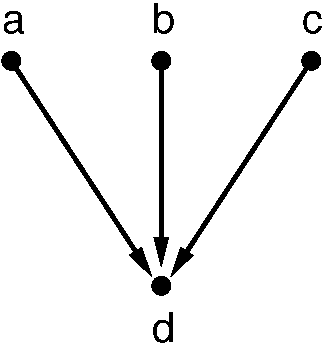
\includegraphics[scale=0.5]{local_function.pdf}
\end{center}
\end{minipage}
\hspace*{0.1in}
\begin{minipage}{0.6\textwidth}
\textbf{Local function}~ $f_d\:$:

\medskip

\begin{itemize}
\item Inputs:~
States of $a$, $b$, $c$ and $d$.  \medskip

\item Output:~ Next state of $d$.
\end{itemize}
\end{minipage}

\bigskip\bigskip

\begin{itemize}
\item The only input to the local function $f_a$ is 
the state of $a$. \\ \medskip

\item A similar comment applies to the local functions
$f_b$ and $f_c$.
\end{itemize}

\bigskip

\noindent
\textbf{Note:}~ The local functions are assumed to be 
\textcolor{dgreen}{\textbf{deterministic}}.
}
%%%%%%%%%%%%%%%%%%%%%%%%%%%%%%%%%%%%%%%%%%%%

\frame[squeeze,containsverbatim]{
\frametitle{An Example of a DAG-SyDS}

\begin{minipage}{0.4\textwidth}
\begin{center}
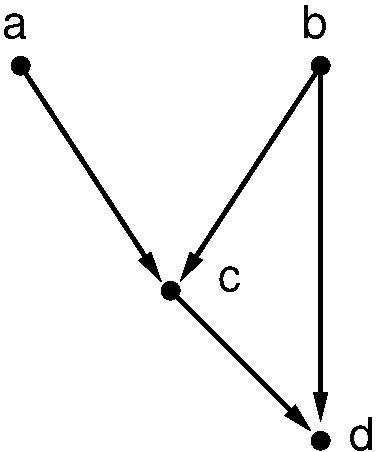
\includegraphics[scale=0.4]{dag_syds_example.pdf}
\end{center}
\end{minipage}
\quad
\begin{minipage}{0.4\textwidth}
\begin{itemize}
\item $\bbb$ = $\{0,1\}$ \medskip
\item $f_a\:$:~ Zero function \medskip
\item $f_b\:$:~ Identity function \medskip
\item $f_c\:$:~ OR function \medskip
\item $f_d\:$:~ AND function
\end{itemize}
\end{minipage}
}
%%%%%%%%%%%%%%%%%%%%%%%%%%%%%%%%%%%%%%%%%%%%

\frame[squeeze,containsverbatim]{
\frametitle{Time Evolution of a DAG-SyDS}
%% \setbeamercovered{dynamic}
\begin{center}
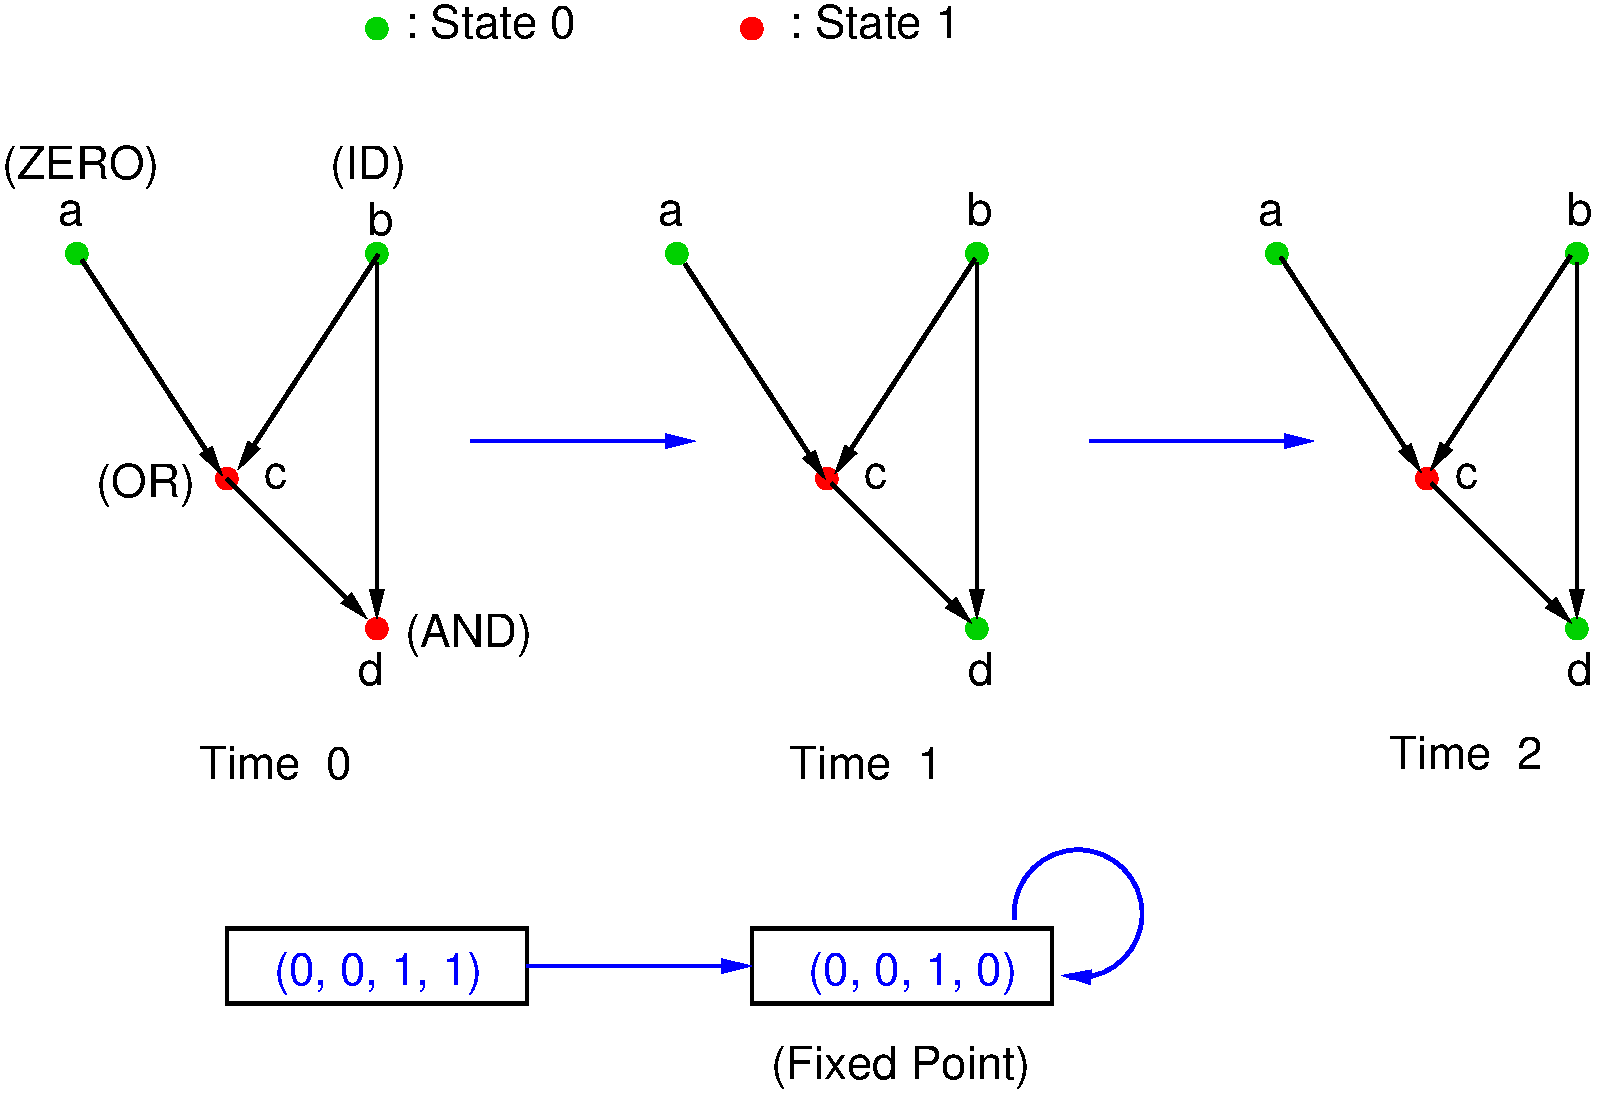
\includegraphics[scale=0.4]{time_evolution.pdf}
\end{center}
}

\frame[squeeze,containsverbatim]{
\frametitle{Some Definitions}
\small{
\begin{itemize}
\item \textcolor{magenta}{\textbf{Configuration}} at time $t$:~ Vector specifying
the state of each node at time $t$.  \medskip

\item \textcolor{magenta}{\textbf{Successor}} of a configuration \calc:~ The configuration
that \textbf{immediately follows} \calc{}
in time evolution. \medskip

\item \textcolor{magenta}{\textbf{Fixed Point}}:~ 
A configuration \calc{} whose successor is \calc{} itself. %\bigskip
\medskip

\item The \textcolor{magenta}{\textbf{phase space}} of a 
discrete dynamical system \cals{} is a \\
\textbf{directed graph} \calp.  \smallskip
  \begin{itemize}
    \item Each node of \calp{} represents a configuration of \cals.  \smallskip
    \item Each directed edge $(x,y)$ indicates that $y$ is the \\ successor of $x$.
  \end{itemize}
\end{itemize}
\medskip
\textbf{Note:}~ The
size of \calp{} is \textcolor{red}{\textbf{exponential}} in the size of \cals.
}
}

\frame[squeeze,containsverbatim]{
\frametitle{Example -- Phase Space of a DAG-SyDS \cals}

\begin{center}
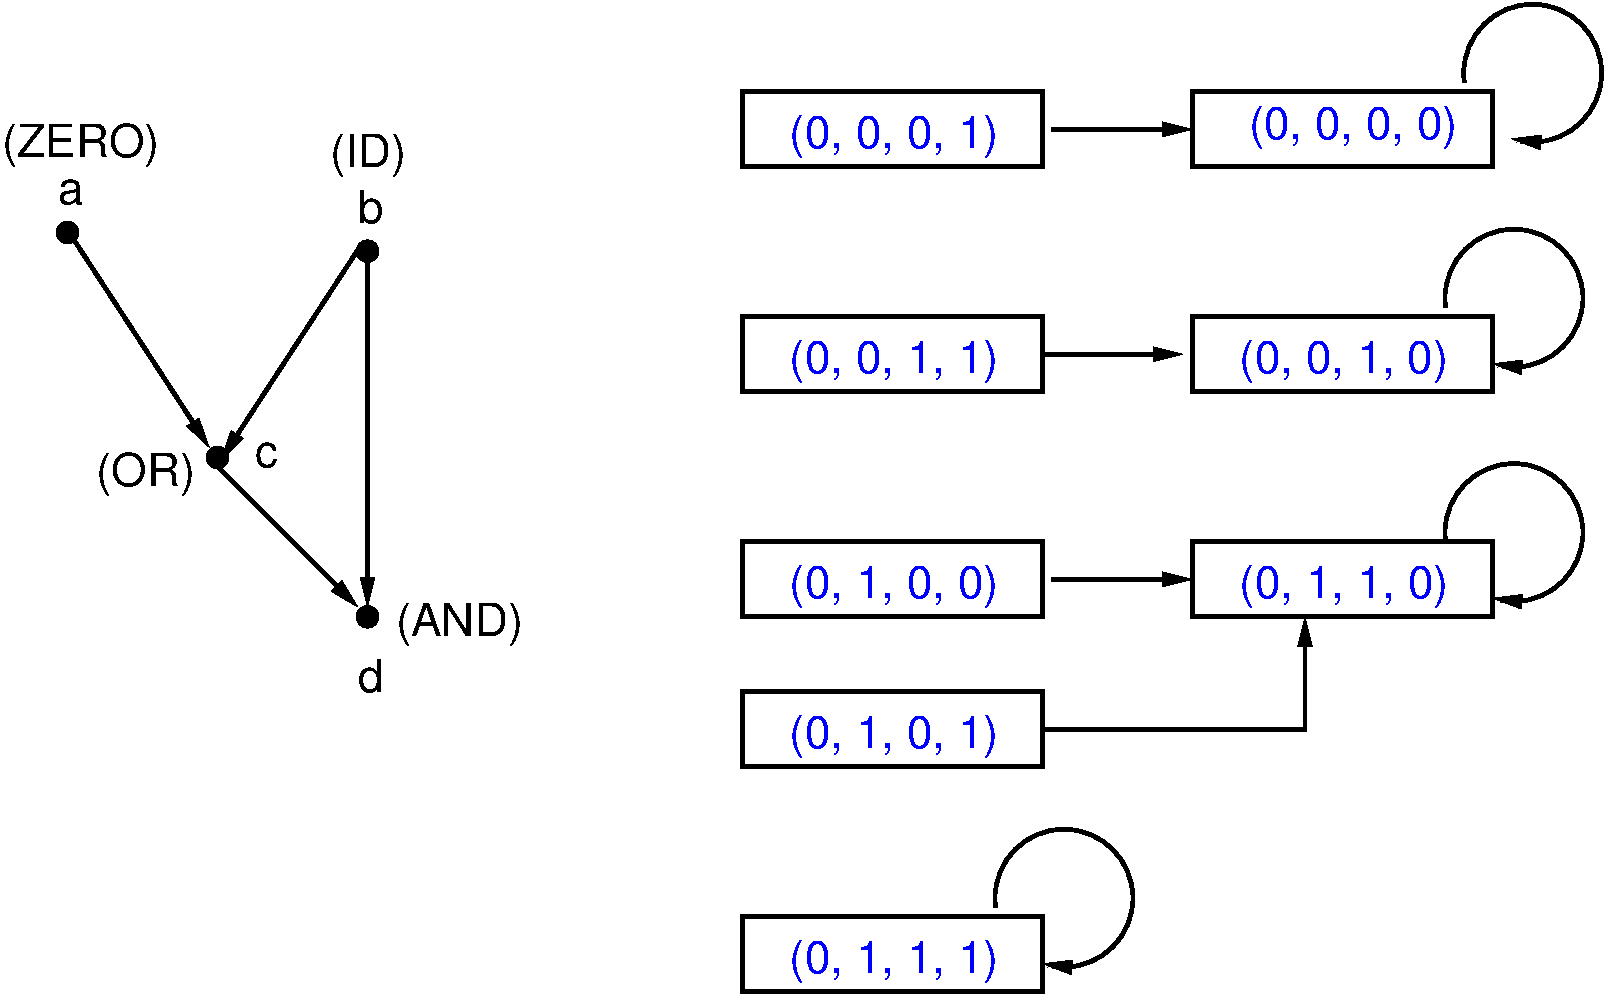
\includegraphics[scale=0.35]{phase_space.pdf}
\end{center}

\medskip

\small{\textbf{Note:}~ Only a part of the phase space is shown.}
}

\frame[squeeze,containsverbatim]{
\frametitle{A Few More Definitions}
\small{
\textcolor{magenta}{\textbf{Transient}}:~ A directed path in the phase space 
ending in\\ a directed cycle. \medskip

\textbf{Example:} The sequence $\langle$C1, C2, C3, C4$\rangle$ in
the following figure. \smallskip

\begin{center}
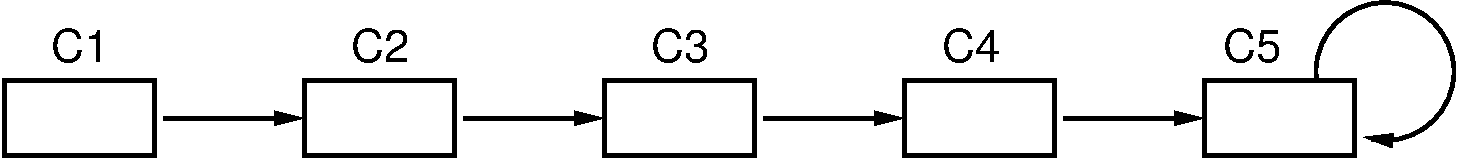
\includegraphics[scale=0.30]{transient.pdf}
\end{center}

\medskip

\textcolor{magenta}{\textbf{Symmetric Boolean Function:}}~ 
A Boolean function whose value remains the same 
when inputs are permuted. (Example: OR, AND, XOR)

\bigskip

\textcolor{magenta}{\textbf{$r$-Symmetric Boolean Function:}}~ 
A Boolean function whose inputs can be partitioned into $r$ classes
so that the function value remains the same 
when inputs in any class are permuted. 

\medskip

\textbf{Note:}~ Each symmetric function is 1-symmetric.
}
}

\frame[squeeze,containsverbatim]{
\frametitle{Motivation: Diffusion Phenomena in Networks}
\small{
\begin{itemize}
\item \textcolor{magenta}{\textbf{Contagion}} processes model many social phenomena \\
      (e.g., propagation of information, influence,
      diseases, trends, etc.). \medskip

\item A well known example: diffusion of opinions in networks
(e.g., \textcolor{blue}{[Auletta et al. 2018, 
Chistikov et al. 2020, Botan et al. 2019, Bredereck \& Elkind 2017]}).
\medskip

\item Usual modeling assumptions:
    \begin{itemize}
        \item Agents in the system have states that vary with time. \medskip
        \item The next state of an agent depends on its current state
              and those of its neighbors (i.e.,
              agent interactions are \textbf{local}).
     \end{itemize}

\medskip

%\item \textcolor{magenta}{\textbf{Threshold-based}} mechanisms commonly used to capture
%     behavior; the behavior of an agent depends
%     on how many of its neighbors are in certain states (e.g.,
%     \textcolor{blue}{[Granovetter~1978, Easley \& Kleinberg~2010]}).

\medskip

\item \textcolor{magenta}{\textbf{Discrete Dynamical Systems:}}~ A formal model for
analyzing contagion phenomena.
\end{itemize}
}}

\frame[containsverbatim]{
\frametitle{Some Analysis Problems for SyDSs}
\small{
\textcolor{magenta}{\textbf{Reachability:}} \medskip

\noindent
\textbf{Given:}~ A SyDS $S$ and
two configurations \calco{} and \calct.  \smallskip

\textbf{Question:}~ Does \cals{} starting from \calco{} 
reach \calct?

\bigskip

\textcolor{magenta}{\textbf{Convergence:}} \medskip

\noindent
\textbf{Given:}~ A SyDS $S$ and
a configuration \calco. \smallskip

\textbf{Question:}~ Does \cals{} starting from \calco{} 
reach a fixed point?

\bigskip

\textcolor{magenta}{\textbf{Convergence Guarantee:}} \medskip

\noindent
\textbf{Given:}~ A SyDS $S$.  \smallskip

\textbf{Question:}~ Does \cals{} reach a fixed point
from \textcolor{dgreen}{\textbf{every}} starting configuration?

\bigskip

\textcolor{blue}{\textbf{Note:}~ The above questions concern
the phase space $\calp(\cals)$ of \cals.}
}}


\frame[containsverbatim]{
\frametitle{Previous Work on Analysis Problems}
%%\small{
%%\textbf{Previous Work:}~ Considered such problems separately \\
%%(e.g.,  \textcolor{blue}
%%{[Barrett et al. 2007, 2006, 2003, 2001]}). 
%%\smallskip

\begin{itemize}
\item Computational intractability of Reachability and 
Convergence problems for dynamical systems on undirected graphs \\
(e.g., \textcolor{blue}{[Barrett et al. 2006, Rosenkrantz et al. 2018]}).
\medskip

\item Computational intractability results for
SyDSs on directed graphs 
\textcolor{blue}{[Ogihara \& Uchizawa: 2017 \& 2020]}. \medskip

\item Computational intractability results in the
AI literature for other dynamical system models: \smallskip

\begin{itemize}
   \item Hopfield neural nets (e.g., 
         \textcolor{blue}{[Orponen: 1993 \& 1994]}). \smallskip
   \item Petri nets (e.g., \textcolor{blue}{[Esparza \& Nielsen 1994]}).
\end{itemize}

\end{itemize}
}

\frame[containsverbatim]{
\frametitle{Previous Work on Analysis Problems (continued)} 

\textbf{Results of} \textcolor{blue}{[Chistikov et al. (AAAI-2020)]}: \medskip

\begin{itemize}
\item SyDSs on directed graphs in the context of diffusion
of opinions. \medskip

\item Each local function is the \textcolor{magenta}{\textbf{majority}} 
function: an agent changes her \{0,1\} opinion only when a majority
of her neighbors have a different opinion.
(This function is 2-symmetric.) \medskip

\item Convergence and Convergence Guarantee problems are 
\cpsp-complete for SyDSs on directed graphs where each local
function is the majority function. \medskip

\item The Convergence problem is efficiently solvable for DAG-SyDSs
regardless of local functions.
\end{itemize}
}

\frame[containsverbatim]{
\frametitle{Other Work Related to DAG-SyDSs} 
\small{
\begin{itemize}
\item For DAG-SyDSs where each local function is a 
\textcolor{magenta}{\textbf{bi-threshold}}
function, Reachability can be solved efficiently \\
(\textcolor{blue}{[Kuhlman et al. 2013]}). \medskip

\item Problem of controlling a SyDS (with external inputs) 
so that the system reaches a desirable configuration can be
solved efficiently when the underlying graph is a 
\textcolor{dgreen}{\textbf{directed tree}} 
(\textcolor{blue}{[Akutsu et al. 2007]}).\medskip

\item Algorithm for inferring the edges of the underlying
graph of a DAG-SyDS from time-series data 
(\textcolor{blue}{[Materassi et al. 2013],}\\ 
\textcolor{blue}{[Cliff et al. 2020]}). \medskip

\item Use of DAG-SyDSs in studying fairness issues for learning
algorithms that interact with an environment
(\textcolor{blue}{[Creager et al. 2020]}).\medskip
\end{itemize}
}
}

\frame[containsverbatim]{
\frametitle{Our Main Contributions}

\textbf{Definition:}~ A \textcolor{magenta}{\textbf{symmetric DAG-SyDS}}
is a DAG-SyDS where each local function is \textcolor{blue}{\textbf{symmetric}}.

\medskip

\begin{enumerate}
\item \textcolor{blue}{Reachability} is \cpsp-complete for symmetric DAG-SyDSs.
%\medskip

  \begin{itemize}
    \item \textbf{Approach:}~ Reduction from Quantified 3SAT (Q3SAT). \medskip

    \item Proof involves two stages.\medskip

   \item \textcolor{blue}{First stage:}~ Use a reduction from Q3SAT to produce 
                a DAG-SyDS where each local function is $r$-symmetric \\
                for some $r \leq 6$.  \medskip

   \item \textcolor{blue}{Second stage:}~ Show that any SyDS where
                each local function is $r$-symmetric for a \textit{fixed} $r$ can be
                simulated by another SyDS where each local function is symmetric.
  \end{itemize}
\end{enumerate}
}

\frame[containsverbatim]{
\frametitle{Our Main Contributions (continued)}

\textbf{Definition:}~ A \textcolor{magenta}{\textbf{monotone DAG-SyDS}}
is a DAG-SyDS where each local function is \textcolor{blue}{\textbf{monotone}}.

\medskip

\begin{enumerate}
\setcounter{enumi}{1}
\item \textcolor{blue}{Reachability} is  efficiently solvable 
for monotone DAG-SyDSs. \medskip

\begin{itemize}
   \item \textbf{Idea:}~ Proof relies on two lemmas. \medskip

   \item For any DAG-SyDS, the length of a transient to a fixed point
         is bounded by the number $L$ of levels in the DAG \\
         (\textcolor{blue}{[Chistikov et al. 2020]}). \medskip

   \item For any DAG-SyDS with monotone local functions, 
         \textcolor{blue}{every cycle in
         the phase space is a fixed point}.
\end{itemize}
\end{enumerate}

\bigskip

\small{
\textbf{Note:}~ For monotone SyDSs on general directed graphs, Reachability 
is \cpsp-complete \textcolor{blue}{[Ogihara \& Uchizawa, 2017]}.
}
}

\frame[containsverbatim]{
\frametitle{Our Main Contributions (continued)}

\medskip

\begin{enumerate}
\setcounter{enumi}{2}
\item \textcolor{blue}{Convergence Guarantee} is  \ccnp-complete 
for DAG-SyDSs with at most \textcolor{dgreen}{\textbf{three}} levels.  \medskip

\begin{itemize}
   \item \textbf{Idea:}~ Reduction from 3SAT. \medskip

%  \item Nodes at Level 0 and Level 1 of the DAG represent variables 
%        and clauses of the 3SAT instance. Level 2 contains a single node. \medskip

\begin{center}
\input{sat_reduction.pdf_t}
\end{center}

\medskip

   \item Local functions ensure that the solution to Convergence
         Guarantee is true iff the given 3SAT instance is 
         \textcolor{dgreen}{\textbf{not satisfiable}}.
\end{itemize}
\end{enumerate}

\smallskip

\small{
\textbf{Note:}~ For SyDSs on general directed graphs, Convergence Guarantee 
is \cpsp-complete \textcolor{blue}{[Chistikov et al. 2020]}.
}
}

\frame[containsverbatim]{
\frametitle{Future Work}

\begin{itemize}
\item Study Reachability and other problems for DAG-SyDSs for other
classes of local functions (e.g., weighted threshold functions). \bigskip

\item Consider additional restrictions on DAGs (e.g., DAGs with bounded
indegree). \bigskip

\item Study DAG-SyDSs where local functions are stochastic.
\end{itemize}

\bigskip\bigskip

\begin{center}
\Huge{\textcolor{blue}{\textbf{Thank You!}}}
\end{center}
}


\end{document}
